\begin{quest}[Reduceerbaarheid]
	Bespreek de twee noties ($A \leq_m B$ en $A \leq_T B$) van reduceerbaarheid, hun verband en op welke manier die noties kunnen gebruikt worden om aan te tonen dat een taal (on)beslisbaar/herkenbaar is.
\end{quest}

Om over te gaan naar de definitie van de reductie van talen, kunnen we best eerst de definitie van Turing-berekenbaar erbij halen (indien we dit niet doen, kunnen we zeker zijn van deze bijvraag).

\begin{theorem}[Turing-berekenbare functie]
	Een functie $f$ heet Turing berekenbaar indien er een Turingmachine bestaat die bij input $s$ uiteindelijk stopt met $f(s)$ op de band.
\end{theorem}

\subsubsection*{Veel-\'e\'en reductie ($\leq_m$)}

\begin{theorem}[Reductie van talen]
	We zeggen dat taal $L_1$ (over $\Sigma_1$) naar taal $L_2$ (over $\Sigma_2$) kan gereduceerd worden indien er een afbeelding $f$ met signatuur $\Sigma^*_1\longrightarrow \Sigma^*_2$ bestaat zodanig dat $f(L_1) \subseteq L_2$ en $f(\overline{L_1}) \subseteq \overline{L_2}$, en zodanig dat $f$ Turing-berekenbaar is. We noteren dat door $L_1 \leq_m L_2$.
\end{theorem}

Tot hiertoe is het al duidelijk wat $L_1 \leq_m L_2$ wil zeggen. Het is nu nog belangrijk om het verband met herkenbaarheid en beslisbaarheid aan te tonen. Dit doen we aan de hand van verschillende, specifiekere stellingen apart te bewijzen. We kunnen achteraf dan de vorige bewijzen gebruiken om ze simpeler te maken.

\begin{theorem}
	Als $L_1 \leq_m L_2$ en $L_2$ is beslisbaar, dan is $L_1$ beslisbaar.
\end{theorem}

\begin{proof}
	Het is belangrijk te weten dat de functie $f$, die elementen uit $L_1$ omzet naar element uit $L_2$, Turing-berekenbaar is. Concreet wil dit zeggen dat we de mogelijkheid hebben om een turingmachine op te stellen met als in put $s_1 \in L_1$ en als output $f(s_1) \in L_2$.\\
	Neem nu dat $L_2$ beslisbaar is, met zijn beslisser $B$. We construeren  nu een machine $F$ die elementen uit $L_1$ omzet (via $f$) naar elementen uit $L_2$, waarna we de beslisser $B$ laten beslissen. Hupsa, de combinatie van $F$ en $B$ is de beslisser van $L_1$ en ook deze taal is dus beslisbaar.
\end{proof}

\begin{theorem}
	Als $L_1 \leq_m L_2$ en $L_2$ is herkenbaar, dan is $L_1$ herkenbaar.
\end{theorem}

\begin{proof}
	Dit bewijs werkt hetzelfde als het voorgaande, om na te gaan dat wanneer $L_2$ beslisbaar is, dat dan ook $L_1$ beslisbaar is. Hier moeten we enkel de beslisser $B$ vervangen door een herkenner $H$.
\end{proof}

\begin{theorem}
	Als $L_1 \leq_m L_2$ en $L_1$ is niet-herkenbaar, dan is $L_2$ niet-herkenbaar.
\end{theorem}

\begin{proof}
	Stel $L_1$ is niet-herkenbaar en $L_2$ wel. We hebben zonet bewezen dat als $L_2$ herkenbaar is, ook $L_1$ herkenbaar moet zijn. Contradictie.
\end{proof}

\begin{theorem}
	Als $L_1 \leq_m L_2$ en $L_1$ is niet-beslisbaar, dan is $L_2$ niet-beslisbaar.
\end{theorem}

\begin{proof}
	Stel $L_1$ is niet-beslisbaar en $L_2$ wel. We hebben zonet bewezen dat als $L_2$ beslisbaar is, ook $L_1$ beslisbaar moet zijn. Contradictie.
\end{proof}

\subsubsection*{Orakels en hi\"erarchie van beslisbaarheid ($\leq_T$)}

Zoals we weten is een Turingmachine een handig hulpmiddel om te bepalen of strings tot een taal horen of niet. We kunnen de machines gebruiken om talen te herkennen, of specifieker, te beslissen. Niet alle talen kunnen echter beslist worden door zo een Turingmachine. Zo is het bijvoorbeeld onmogelijk om een Turingmachine op te stellen die de taal $A_{TM}$ beslist.
\\\\
Dit zorgt er voor dat we op zoek moeten gaan naar een betere machine die naast het beslissen van de al besliste talen, ook andere talen kan beslissen. De nieuwe machine moet dus krachtiger zijn. Het resultaat is een orakelmachine.
\\\\
Een orakelmachine is een uitbreiding op de Turingmachine, die een orakel bevat. Je kan een orakel bekijken als een black box waar de Turingmachine vragen een kan stellen. In theorie is een orakel eigenlijk een soort bitmap, of anders gezegd een rij van booleans. Stel we ordenen alle strings volgens de lexicografische orde met kortere strings eerst. Elke string op index $i$ komt nu overeen met een booleaanse waarde in de bitmap, die ook gealloceerd is op locatie $i$. Indien de string op een bepaalde locatie tot een gegeven taal $L$ behoord, dan zal de overeenkomstige booleaanse waarde op $true$ staan. Indien dit niet het geval is, blijft de waarde op $false$.
\\\\
De werking van een orakelmachine is nu heel eenvoudig. Het krijgt als input een string $s$. De machine vraagt nu aan het orakel of de string tot een taal behoort. Het orakel is in staat om de string om te vormen naar de index in de rij volgens de lexicografische volgorde en raadpleegt de overeenkomstige booleaanse waarde in de bitmap. Is die waarde $true$, dan accepteert het orakel de string $s$. Indien de waarde $false$ is, dan wordt de string $s$ geweigerd. Een orakelmachine waarvan de bitmap een configuratie heeft voor een bepaalde taal $L$ te beslissen, noemen we $O^L$.

\vspace{3mm}
\begin{figure}[h!]
  \centering
      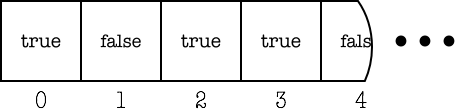
\includegraphics[width=0.5\textwidth]{./img/oracle}
  \caption{Simpele voorstelling van een orakel (bitmap).}
\end{figure}
\vspace{3mm}

Een orakel kan voor vele problemen gebruikt worden. Het halting probleem is hier echter maar \'e\'en enkel voorbeeld van. Vaak wordt een orakel gebruikt om op een abstracte manier een antwoord te krijgen op een bepaalde vraag. Deze vraag kan zelfs onoplosbaar zijn.

\begin{theorem}[Turingreduceerbaar]
	Een taal $A$ is Turingreduceerbaar naar taal $B$, indien $A$ beslisbaar is relatief t.o.v. $B$, t.t.z. er bestaat een orakelmachine $O^B$ die $A$ beslist. De notatie is $A \leq_T B$.
\end{theorem}

Dit is inderdaad zeer gelijkend op het eerste deel van deze vraag. In plaats van een beslisser voor $B$ te hebben, die $A$ ook beslist, gebruiken we nu een orakelmachine. Deze machine is dan een theoretisch hulpmiddel dat we kunnen gebruiken om onze kennis toe te passen op meerdere talen. Deze kunnen we echter in realiteit niet implementeren zoals we net beschreven hebben.

\begin{theorem}
	Indien $A \leq_T B$ en $B$ is beslisbaar, dan is $A$ beslisbaar.
\end{theorem}

\begin{proof}
	De definitie zegt ons dat $A \leq_T B$ enkel geldt indien we een orakelmachine $O^B$ hebben dat $B$ \'en $A$ beslist. Dit is dus volledig afleidbaar van de definitie. Of anders: stel dat $B$ beslisbaar is en $A$ niet. Dan hebben we een orakel $O^B$ dat (theoretisch) $B$ beslist, maar niet $A$ (want deze is niet beslisbaar). Dit is meteen een contradictie met de definitie.
\end{proof}

\begin{theorem}
	Indien $A \leq_m B$ dan is ook $A \leq_T B$. M.a.w. $\leq_m$ is fijner dan $\leq_T$.
\end{theorem}

Dit is vanzelfsprekend indien we beseffen dat het orakel een theoretische uitbreiding is op de Turingmachine. We gebruiken de Turingmachines om talen te herkennen of the beslissen. Het is mogelijk zo een machine te implementeren in een taal naar keuze. Er is echter een grens op het aantal talen dat we kunnen beslissen, aangezien een aantal in een oneindige lus kunnen komen tijdens het beslissingsproces. Dit is een probleem dat we in de praktijk kunnen tegenkomen. Een theoretische oplossing daarvoor is de orakelmachine. We kunnen deze machine wel gebruiken om theoretisch verder te redeneren. Dit will zeggen dat het orakel alle talen beslist dit een Turingmachine kan beslissen, plus de talen die een turingmachine niet kan beslissen (oneindig lus). Hierdoor is $A \leq_m B$ fijner dan $A \leq_T B$.
